\documentclass[10pt]{beamer}

% Balíčky
\usepackage[czech]{babel}
\usepackage{bchart}

% Makra
\newcommand{\resources}{Resources/}

% Nastavení beamer titlepage
\title{Vývoj akční videohry zasazené do prostředí FM}
\subtitle{Bakalářský projekt}
\author{Radek Mocek}
\date{}

% Beamer template
\input{\resources beamerTemplate}

% Začátek prezentace
\begin{document}
	
	% Titulní strana
	{
	\setbeamertemplate{footline}{} % Titulní strana bez patičky
	\frame[noframenumbering]{\titlepage} % Nepočítat do celkového počtu framů
	}
	
	% Obsah
%	\begin{frame}{Obsah prezentace}
%		\tableofcontents
%	\end{frame}	

	% Slide 0 :: Zadání
	\section{Zadání} % Tohle je zde kvůli případnému obsahu
	\begin{frame}{Zadání} % Slide a jeho napdpis
		\begin{enumerate} \setlength\itemsep{10pt} % Číslovaný seznam
			\item Proveďte rešerši nástrojů pro tvorbu 2D videoher s využitím Unity engine. Prozkoumejte jejich funkce, výhody a nevýhody a jak se dají použít pro vaše potřeby.
			\item Navrhněte koncept herní mechaniky pro 2D top-down videohru.
			\item Vytvořte jednoduchý systém umělé inteligence pro nepřátelské jednotky ve hře,	který bude řízen stavovým automatem.
			\item Implementujte demonstrativní videohru zasazenou do prostředí budovy FM TUL.
			\item Výslednou videohru kriticky zhodnoťte a navrhněte případné rozšíření či vylepšení.
		\end{enumerate}
	\end{frame}

	% Slide 1 :: Motivace
	\section{Motivace}
	\begin{frame}{Motivace}
		\begin{itemize}\setlength\itemsep{10pt} % Nečíslovaný seznam
			%\item Záliba ve videohrách
			\item Rozmanitost herního vývoje
			\item Unity $\implies$ C\#
		\end{itemize}
	\end{frame}
	
	% Slide 2 :: Unity obecně
	\section{Unity}
	\begin{frame}{Unity}
		\begin{itemize}\setlength\itemsep{10pt}
			\item Herní engine, 2D i 3D tvorba
			\item 2005, Unity Technologies, closed source
		\end{itemize}
		\vfill
		\begin{bchart}[max=108,plain,unit=\ 000,scale=1.2]
			\bcbar[text=Unity,color=gray!40!white]{108}
			\bcbar[text=Construct,color=teal!40!white]{32}
			\bcbar[text=GM:S,color=green!40!white]{15}
			\bcbar[text=Godot,color=blue!40!white]{14}
			\bcxlabel{Počet projektů v daném enginu na itch.io (zaokrouhleno na tisíce)}
		\end{bchart}
	\end{frame}
	
	% Slide 3 :: Unity obrázek
	% >> Zmínit komponenty, C#, IDE
	\begin{frame}[plain]
			\makebox[\linewidth]{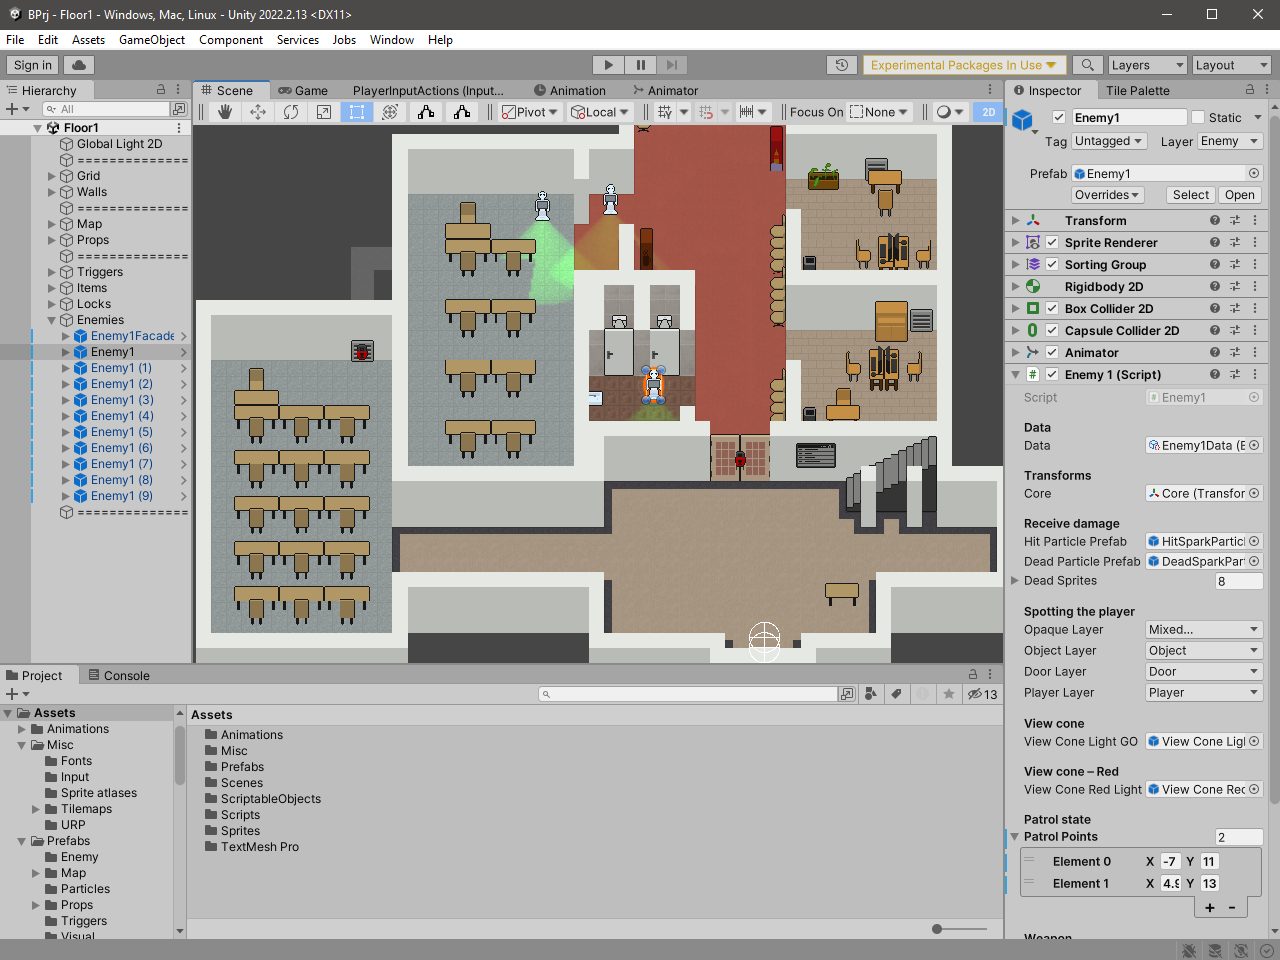
\includegraphics[width=\paperwidth]{Images/Unity}}
	\end{frame}
	
	% Slide 4 :: Unity 2D showcase
	\begin{frame}[plain]
		\makebox[\linewidth]{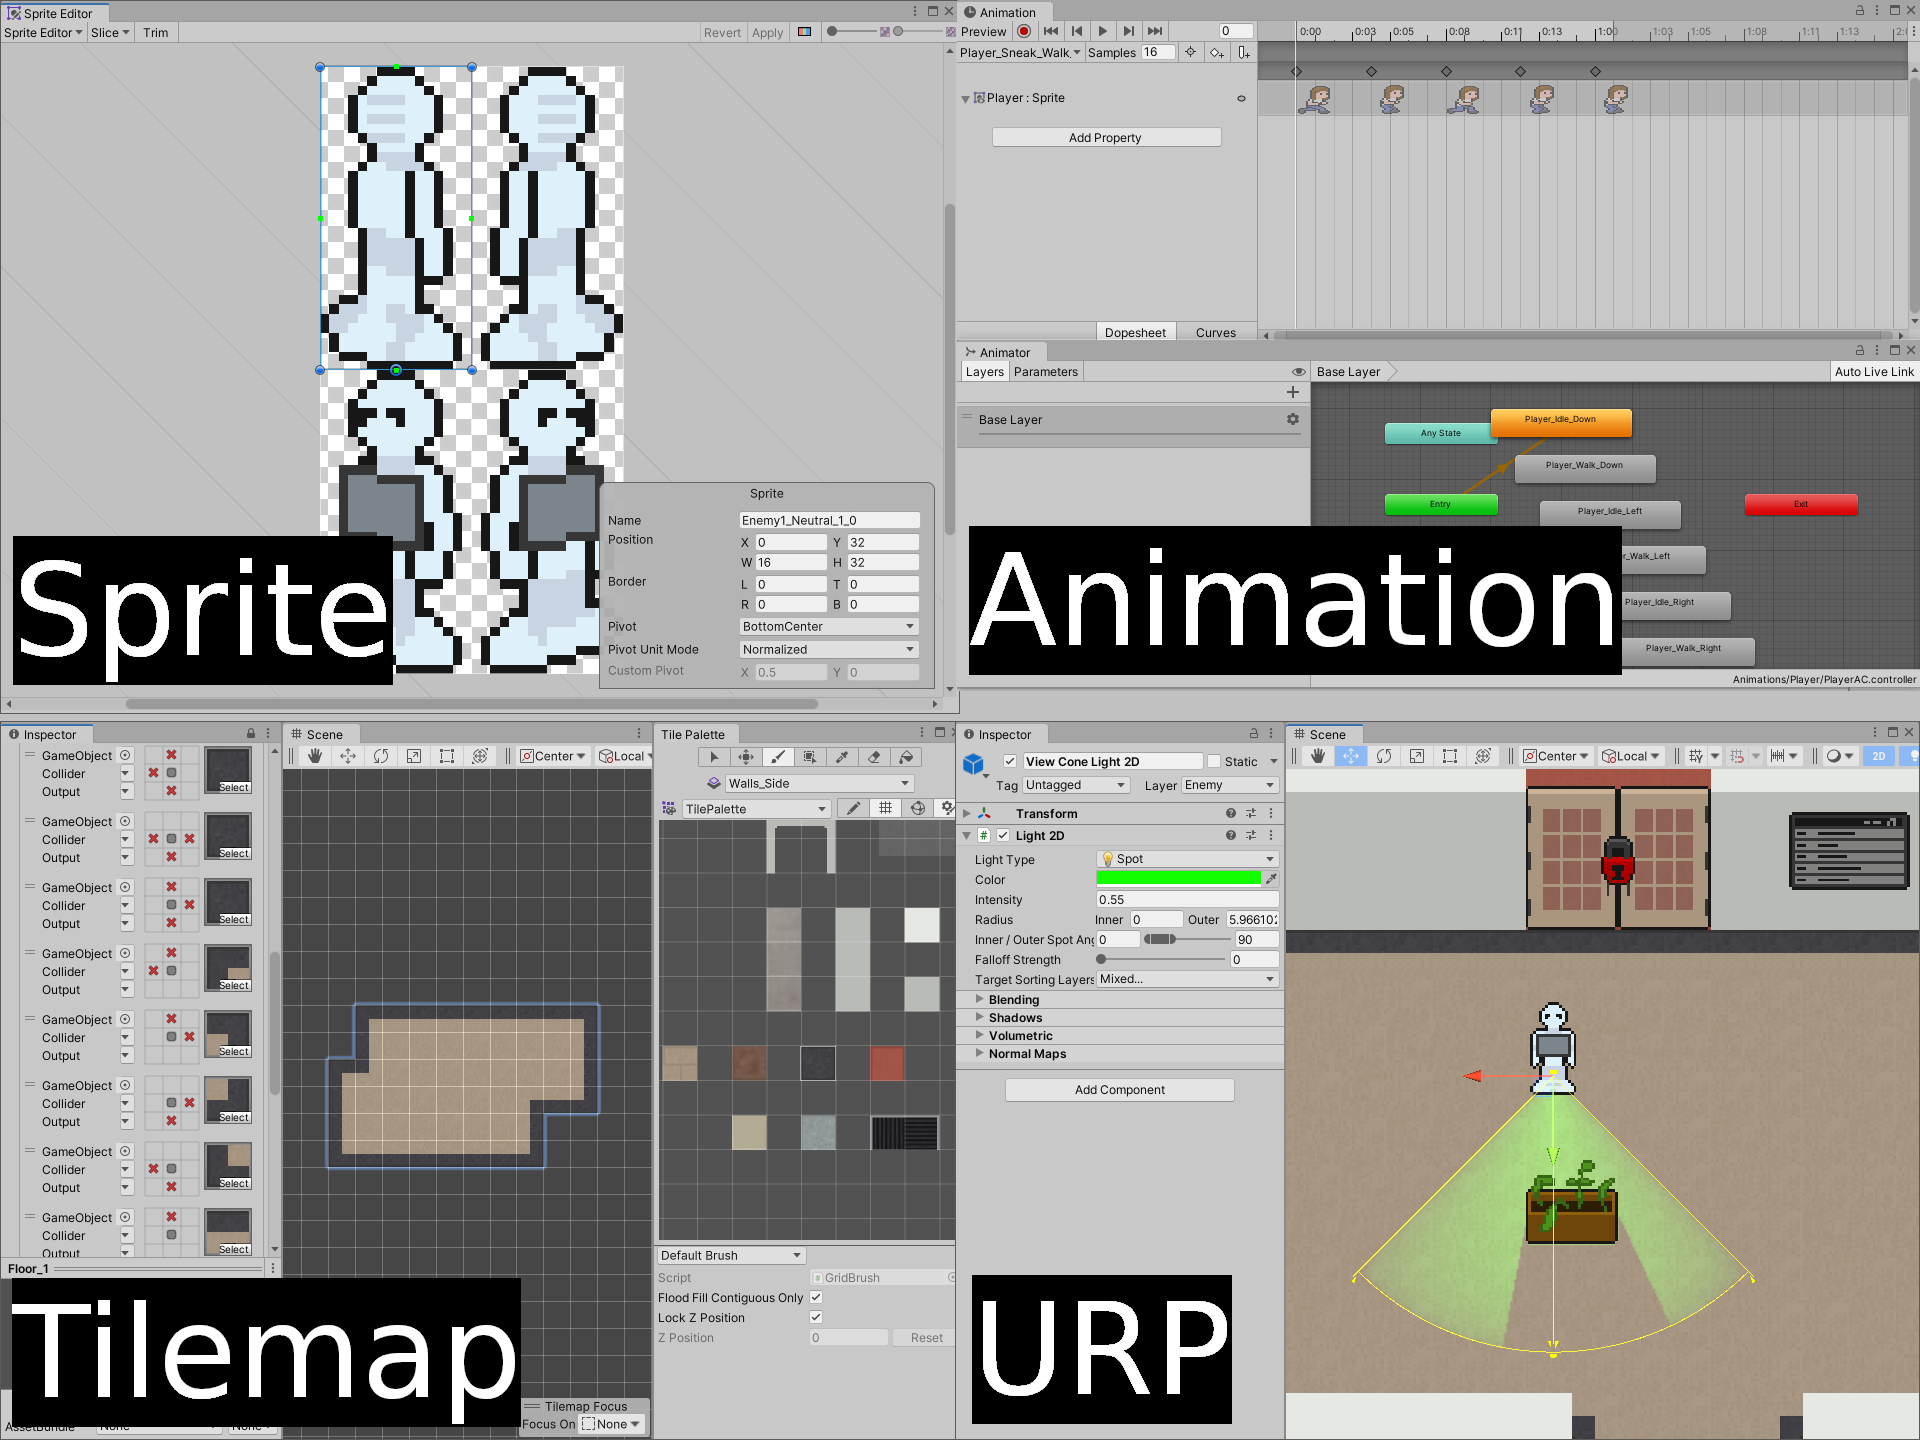
\includegraphics[width=\paperwidth]{Images/UnityShowcase}}
	\end{frame}
	
	% Slide 5 :: Návrh
	\section{Návrh}
	\begin{frame}{Návrh}
		\begin{itemize}\setlength\itemsep{10pt}
			\item Příběh
			\item Vizuální stránka
			\begin{itemize}
				\item Pixel art – jednoduchost, rychlost
				\item Top-down perspektiva
			\end{itemize}
			\item Žánr
			\begin{itemize}
				\item Akční
				\item Stealth
			\end{itemize}
		\end{itemize}		
	\end{frame}
		
	% Slide 6 :: Návrh FSM
	\section{Návrh – stavový automat}
	\begin{frame}{Návrh – stavový automat}
		\begin{figure}[h]
			\centering
			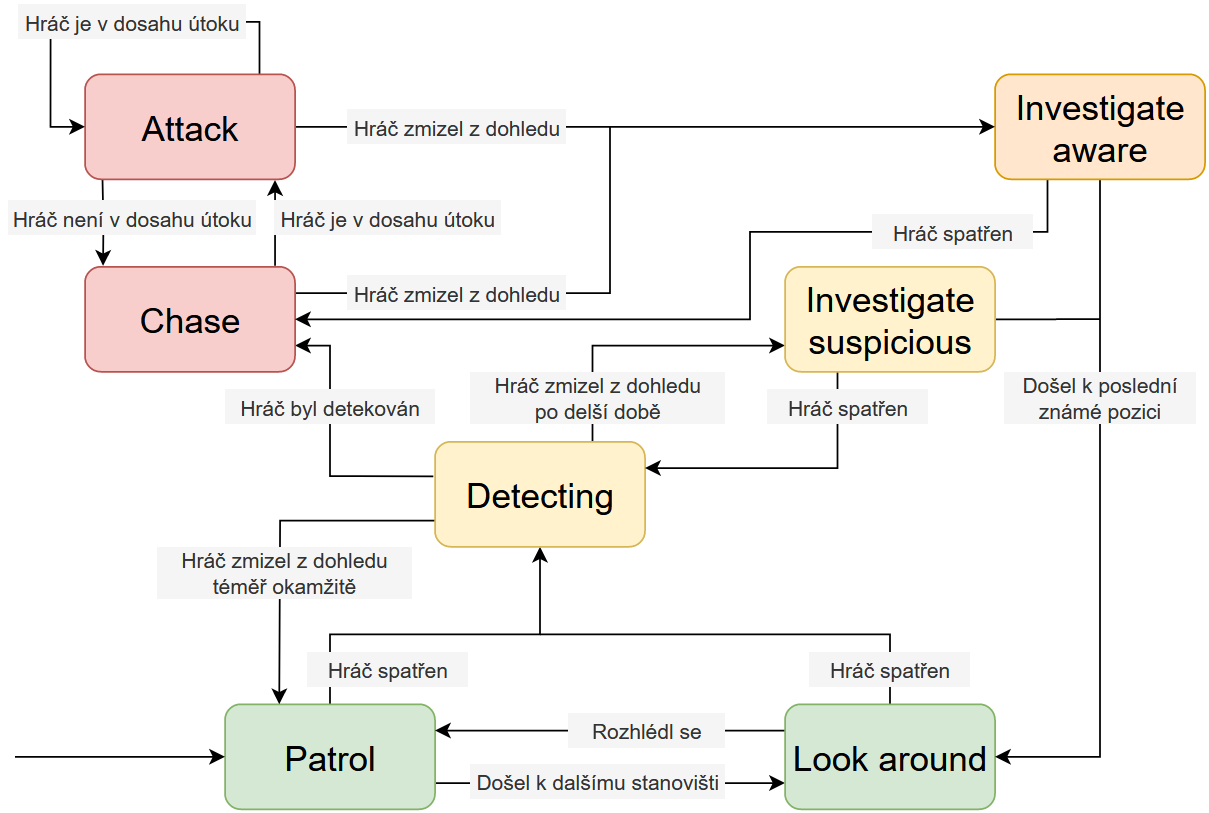
\includegraphics[width=\textwidth]{Images/FSM}
		\end{figure}
	\end{frame}
	
	% Slide 7 :: Implementace
	\section{Implementace}
	\begin{frame}{Implementace}
		\begin{itemize}\setlength\itemsep{10pt}
			\item Grafika – GIMP, problémové animace
			\item Postava hráče – RigidBody2D, stavový automat
			\item Tvorba mapy – tilemap, problémy s perspektivou a URP
			\item Jednotka nepřítele – stavový automat, A*
		\end{itemize}
		\vfill
		\begin{figure}[h]
			\centering
			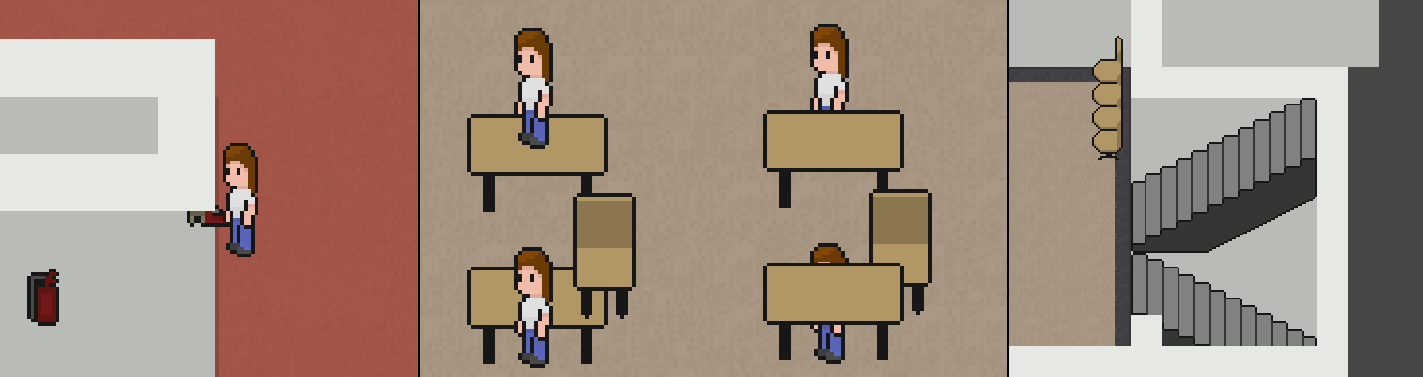
\includegraphics[width=\textwidth]{Images/Perspective}
		\end{figure}
	\end{frame}
	
	% Slide 8 :: Implementace FSM
	\section{Implementace – stavový automat}
	\begin{frame}{Implementace – stavový automat}
		\begin{figure}[h]
			\centering
			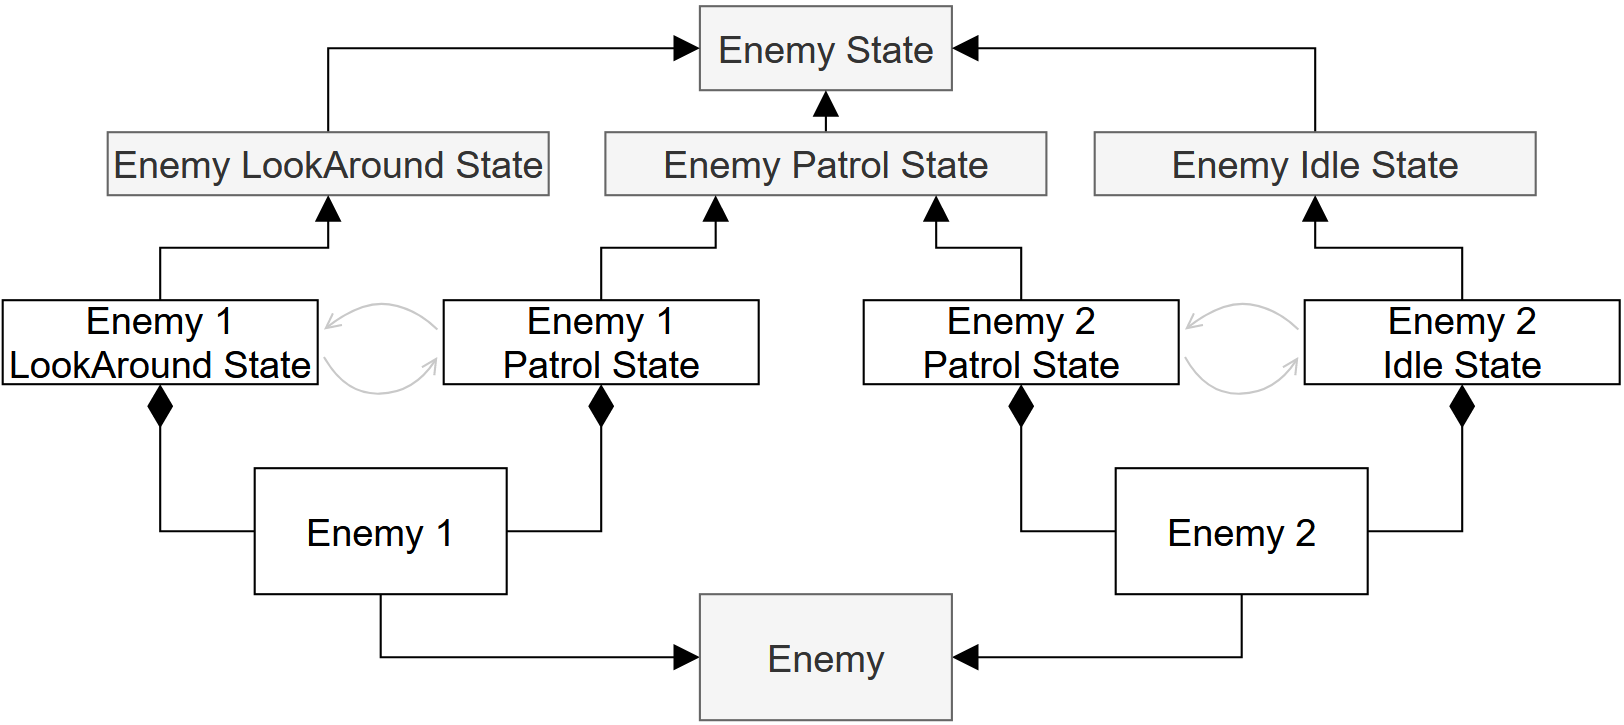
\includegraphics[width=\textwidth]{Images/FSM_Specific}
		\end{figure}		
	\end{frame}

	% Slide 9 :: Závěr
	\section{Závěr}
	\begin{frame}{Závěr}
		\begin{itemize}\setlength\itemsep{10pt}
			\item $+$ Grafický styl
			\item $+$ Stealth
			\item $+$ Implementace stavového automatu
			\item $-$ Audio
			\item $-$ Soubojový systém
			\item $-$ Přístupnost
		\end{itemize}
	\end{frame}

	% Děkuji za pozornost
	{
	\setbeamertemplate{footline}{} % Závěr bez patičky
	\begin{frame}[noframenumbering] % Nepočítat do celkového počtu framů
		Děkuji za pozornost
	\end{frame}
	}
	
\end{document}